
\chapter{Introduction}


Manipulating the formation of a condensed phase is a critical part of both nature and technology. From molluscs controlling crystal formation~\cite{de-yoreo:03}, increasing the solubility of drugs~\cite{hancock:00}, plastics~\cite{bennemann:99}, silicon in photovoltaic cells\tocite, and many other materials that we rely on every day~\cite{kim:07}. As the devices we use become smaller the need to understand the processes that form them becomes more important. A complete theory of glass formation is still elusive and our ability to control crystal formation is far from what is available to nature. To better understand the formation of the solid phase, we need an understanding of the molecular rearrangements that take place as we move from a molecular liquid, through a supercooled liquid to either a glass or molecular crystal.

The goal of my project is to explore how fundamental features of molecular shape - asymmetry and concavity - influence the properties of the various condensed phases; liquid, crystal, glass and supercooled-liquid. This requires the characterisation of a new set of molecular models for computer simulation. I will be addressing how the degree of concavity in the molecular shape determines the dynamics of rotations and translations in the low temperature liquid phase and, the effect that molecular shape has on the process of crystallisation.

To fully understand these concepts we first need to understand the bulk properties of the condensed phases and their formation.


\section{Molecular Crystals}
\label{sec:molecular crystals}

The unit cell is the building block of a crystal. As such it is a useful tool to be able to describe the type of crystal. While it is common to refer to a crystal structure type in terms of a example material e.g. \ce{CsCl} structure, or \ce{NaCl}, Zinc blende and many others, these names do not directly inform us of the properties of the underlying unit cell. The complete descriptor of the unit cell is the \emph{space group}, a set of symmetry operations that act on the molecules of a unit cell. This is a more formal approach to describing one crystal in terms of another and allows comparison of unit cells based on their properties, such as the number of symmetry operations within a unit cell. It is also possible to look at the distribution of crystal structures over the unit cells, with a distribution among a large number of space groups for inorganic crystals with no space group representing more that \SI{8}{\percent} of crystal structures~\cite{ursov:09}. On the other hand molecular crystals are far more specific in the space groups that they occupy, with the $P2_{1/c}$ space group contains over a third of all molecular crystals~\cite{brock:94} and the five most populous space groups contain \SI{75}{\percent} of all molecular crystals.

Understanding the difference between metallic and molecular crystals molecules requires the simplification of the problem into two dimensions. Using two dimensions has many benefits over a three dimensional system. Computations are far quicker in two dimensions, the complexity of the calculation is often to the power of the dimension, instead of dealing with $n^3$ calculations there are only $n^2$; a big difference when $n$ is large. The visualisation of a two dimensional system on a two dimensional interface such as a computer monitor or a piece of paper is also simpler, being able to directly observe ongoing processes. This makes visual identification of a pattern or property that incites Issac Asimov's famous ``that's funny'' response far more likely. Another benefit of working in 2D is that there are only 17 \emph{wallpaper groups}, the 2D equivalent of space groups. Wallpaper groups are constructed in the same way as space groups and 2D makes it easier to identify the symmetry operations~\figref{wallpaper}. In a similar manner to 3D we can group all the 2D molecular shapes that have been studied into their wallpaper groups, there are two wallpaper groups that contain the vast majority of molecules, the p2 and the p2gg wallpaper groups~\cite{plass:07}. As a general guideline for the packing of 2D molecules without central symmetry, \textcite{torquato:12} note that the molecules tend to pair such that the pair will have an inversion center~\figref{molecule pair}. This concept of an inversion center also applies to the 3D system, the P2$_1$/c space group also has an inversion center and generally inversion centers are favoured~\cite{brock:94}.

\begin{figure}
    \centering
    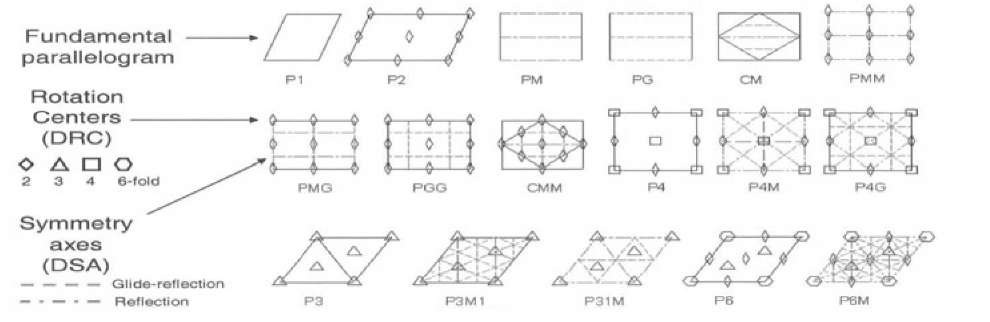
\includegraphics[width=\textwidth]{wallpaper_groups}
    \caption{Showing some of the wallpaper groups and the symmetry operations that comprise them.}
    \source[\ccpd]{gagern:08}
    \label{fig:wallpaper}
\end{figure}

\begin{figure}
    \centering
    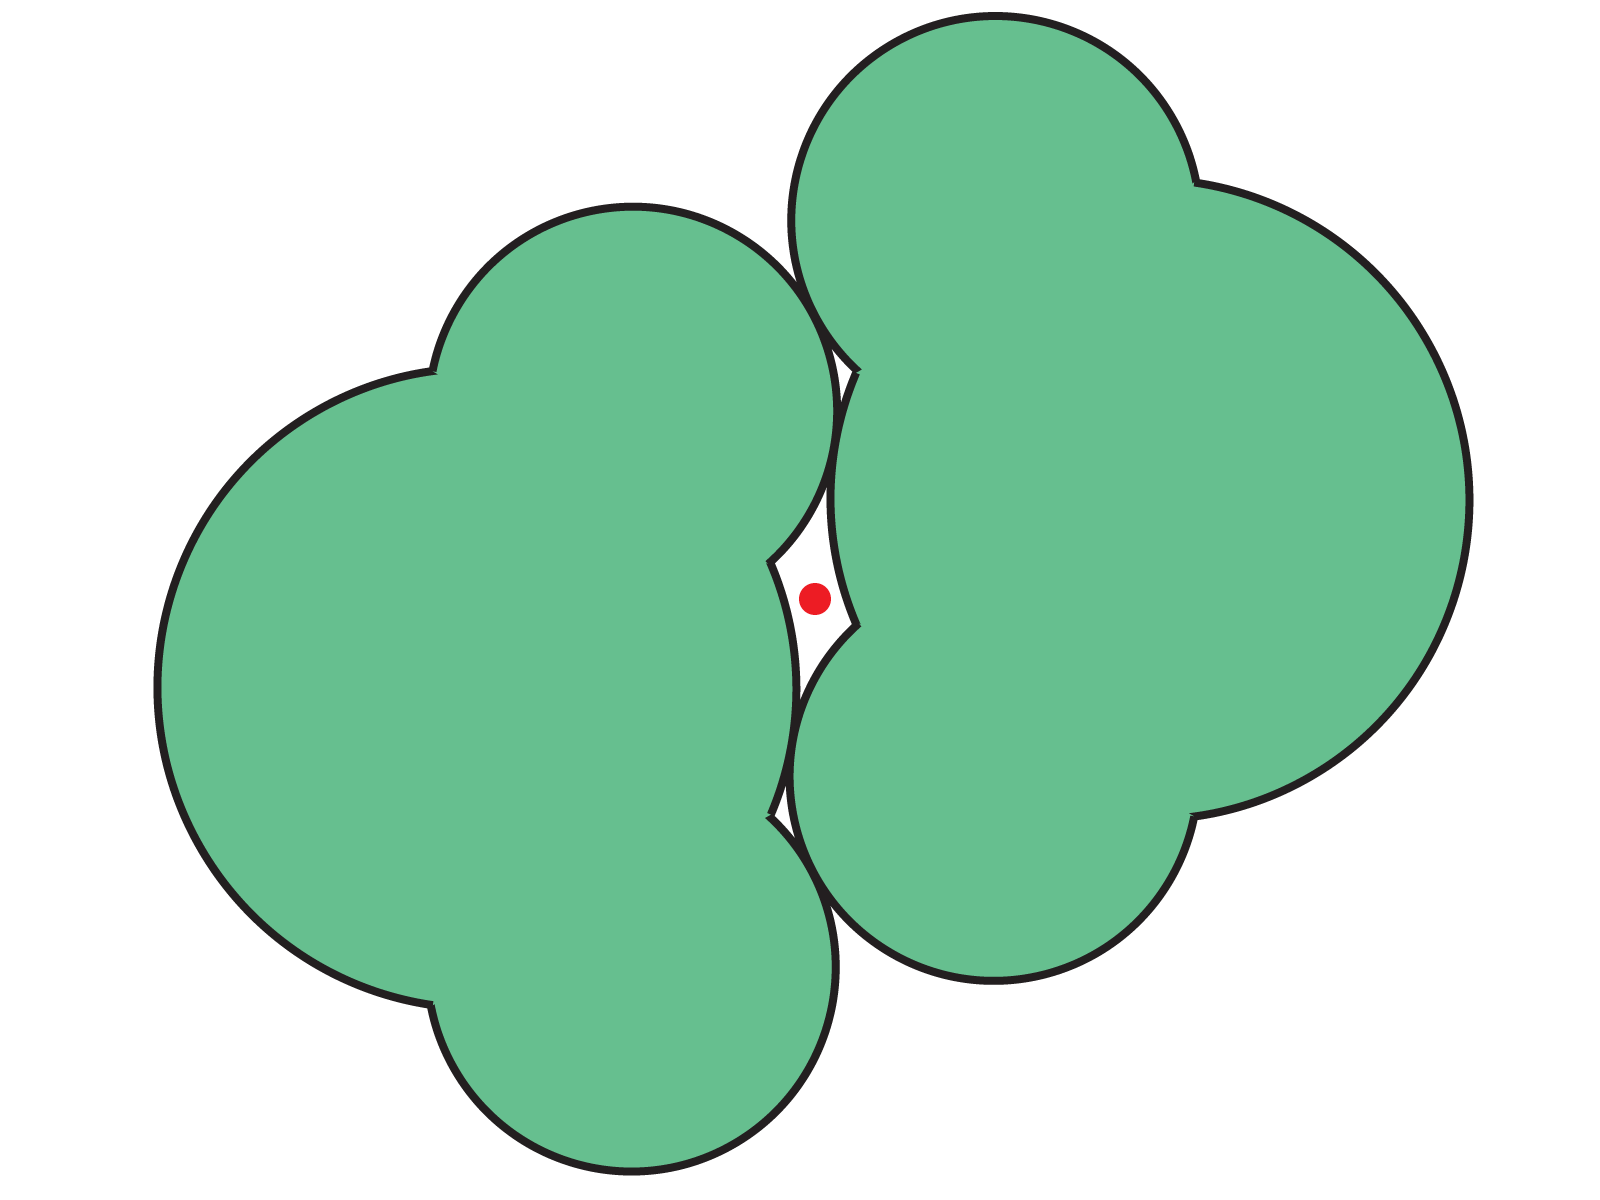
\includegraphics[width=0.5\linewidth]{pairing}
    \caption{When molecules are non centrally symmetric they tend to pair creating an inversion center (shown in red).}
    \label{fig:molecule pair}
\end{figure}

The way that molecular crystals pack space is an important problem in simulating crystal structures. One of the methods used to find the optimal crystal structure is to model the molecule as an arrangement of hard spheres and find the arrangement of molecules that occupies the largest volume of space~\cite{kitaigorodskii:73}, also known as the \emph{packing fraction}. The simplest example of this is packing spheres, to which Kepler proposed that the hexagonal close packed structure was the most efficient in 1611~\cite{kepler:1611}. The hexagonal close packed structure has the same packing fraction as the face centered cubic structure despite being structurally distinct. While these structures have been considered the best possible packing of spheres in space for hundreds of years there has not been a mathematical proof until recently. In 2005 \textcite{hales:05} published a 400 page proof of this problem of which mathematicians were \SI{99}{\percent} certain was correct. Nearly 10 years later Hales {\em et al.}~\cite{hales:14} announced the completion of a project to completely satisfy the proof, using computers to check all possible configurations. 

\begin{figure}
    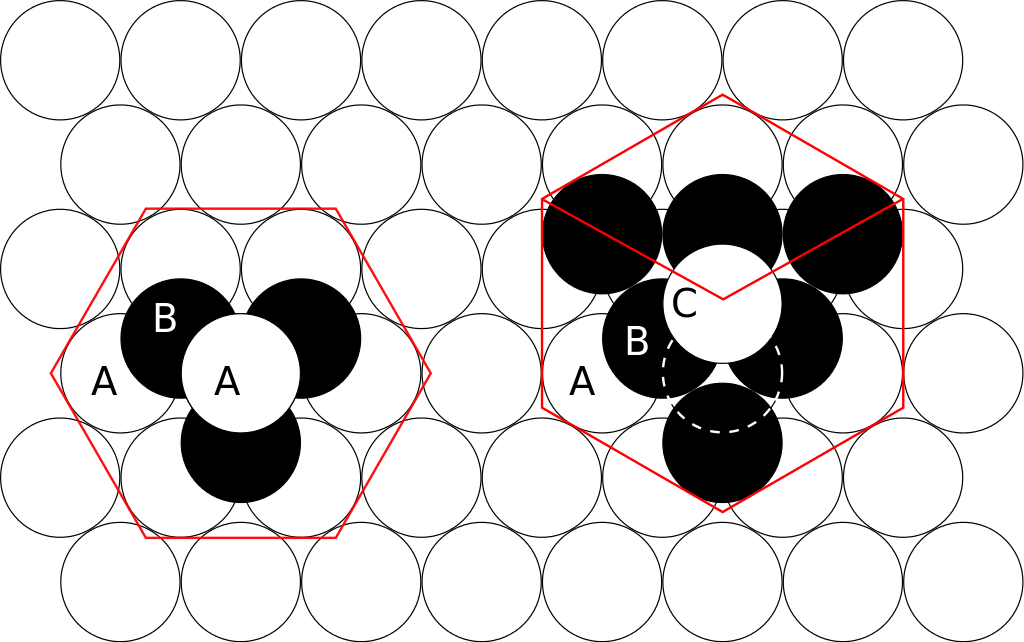
\includegraphics[width=\textwidth]{close-packing}
    \caption{There are two structurally distinct closest packings of spheres, the hexagonal close packed structure and the cubic close packed structure}
    \source[\ccpd]{twisp:08}
    \label{fig:sphere packing}
\end{figure}

If finding a proof for the simplest of shapes was so difficult, how hard is it going to be to find closest packings for arbitrary molecules. While having a mathematical proof of the closest packed structure is nice, it is not necessary to perform useful chemistry, using the closest known packed structure is a reasonable, and often correct alternative. Without the requirement for proof of correctness the problem of finding the closest known packing of arbitrary molecules becomes far simpler. The degrees of freedom of the particles can be considered a multidimensional space with the value at each point in space being the packing fraction, finding the solution is now a case of finding the global minimum of this multidimensional function. Finding the global minimum of a function is a problem that appears in many fields, including computer science. As such there are a number of algorithms that can be used in an attempt to find the global minimum~\cite{press:07}. It should be noted that the only method that guarantees finding the global minimum is to evaluate the packing fraction at every possible configuration. This is not computationally possible for any reasonably sized system, the number of points required scales exponentially with the number of molecules, quickly running into calculations that would take longer than the age of the universe. Many of these approximations use the concept of simulated annealing~\cite{kirkpatrick:83} which stems from the process of glass formation. This is the process by which the configuration is given an amount of energy to move around the configuration space, moving out of a configuration that has a low packing fraction happens with a high probability, while moving out of a well where the packing fraction is high occurs with low probability. The probability of the configuration moving scales with the energy, as the energy is slowly reduced only the best configurations are sampled. If the energy is reduced slowly enough the global minimum is the final configuration, however there is no way to determine beforehand what slowly enough is.

Along with categorising the crystal structure, the unit cell of a crystal structure is also responsible for many of the properties of the resulting material including the shape, physical properties, magnetic properties, conductivity, piezoelectric properties and many more. As we increase the temperature of a crystal these properties degrade from the additional disorder until we reach the liquid phase.

\section{Molecular Liquids}

The liquid phase is defined by its incompressibility and its ability to flow. There are two forces, a long range attractive and a short range repulsive, that define this behaviour. The ability to flow is comes from the energy of the particles, they have enough energy to move out of their local environments, but not enough to escape the attractive forces of the neighbouring particles as they flow around them. This attractive force is integral to the liquid phase, if the force is too short range or not present then the liquid phase does not exist~\cite{tejero:94}, only the solid and gas phases will form. When considering the process that occurs when a liquid flows, molecules must move away from their optimal position and around neighbouring molecules. If the attraction is too small at these larger distances there is nothing stopping the molecule flying off and becoming a gas. The other important force in a liquid is the repulsive force which is responsible for the structure of the liquid. A common measure of the structure of the liquid phase is the \emph{pair distribution function}~\figref{radial distribution} denoted $G(r)$ and given by
\begin{equation}
    G(r) = \frac{1}{N\rho} \sum_i^N \sum_{j\ne i}^N \delta[ r - r_{ij}]
\end{equation}
where $N$ is the number of particles $\rho$ is the number density and $r_{ij}$ the separation of two particles. In essence it maps the probability of finding molecules at a distance $r$ from any particle, however unlike a probability the radial distribution function is normalised to $N-1$ where $N$ is the total number of particles in the system. It can also be expressed as the term that when multiplied by the number density $\rho$ gives the local density around a particle. The radial distribution function gives a very clear distinction between between the crystal, and liquid~\figref{radial distribution}. In the liquid phase phase we can see there is a region of excluded volume at small $r$, this is the result of the repulsive force, the apparent size of the molecule. Beyond the excluded region there is a sharp peak corresponding to the shell of nearest neighbours around the central molecule. It is the excluded region and short range ordering that results in the incompressibility, there is nowhere for the particles to move upon compression because of the repulsive force. The final part of the radial distribution function is the long range behaviour, for liquids there is no long range ordering, while for crystals there are peaks out to very large $r$. The radial distribution function is a property computed for a system where it is easy to calculate the distance between each particle, for experimental systems this is not possible. The strength of the radial distribution function is that is can be linked to a directly measurable quantity, the \emph{static structure factor} by a Fourier transform
\begin{equation}
    S(q) = 1 + \rho \int [G(r)-1]\,\e^{ikr}\, \d r
\end{equation}
The static structure factor can be experimentally determined by taking the x-ray diffraction pattern of a sample, providing a direct comparison between experimental and theoretical systems. Along with the structural differences between a liquid and a crystal there are also significant dynamical differences.

\begin{figure}
    \todofigure{Radial distribution functions}
    \caption{}
    \label{fig:radial distribution}
\end{figure}

Two characteristic dynamic properties of a liquid are the viscosity and diffusion. The viscosity ($\eta$) of a liquid is a property of the bulk liquid measured in units of \emph{poise} (\si{\poise}). The viscosity is a temperature dependent quantity, following an Arrhenius relationship
\begin{equation}
    \eta = \eta_0\, \e^{-E_a/(\boltzman T)}
\end{equation}
where $\eta_0$ is the viscosity at a known temperature $T_0$, \boltzman is the Boltzman constant, and $E_a$ is the activation energy. In this case the activation energy can be considered the energy required to move past the nearest neighbours. The Arrhenius relation holds because this activation energy remains constant throughout the temperature range. The other dynamic property is diffusion, this is a property of averaged over individual molecules. At short times the mean squared displacement (MSD) is dominated by ballistic motion from the local vibrations of particles. However at longer times we get a relation
\begin{equation}
    \langle |\Delta \vect r|^2 \rangle = \frac{6\boltzman T}{m\zeta} = 6Dt
\end{equation}
where $\Delta \vect r$ is the distance between $r$ and $r_0$, $T$ is the temperature, $m$ is the molecular mass and the angle brackets denote averaging over all molecules. The diffusion constant $D$ can be defined as $D = \boltzman T/m\zeta$ simplifying the equation. The factor of 6 is a property of a three dimensional system, for a two dimensional system a factor of 4 is used instead. When dealing with molecules, along with translational motion, rotational motions are also important.


\towrite{rotational relaxations}
\begin{itemize}
    \item Rotational relaxation of OTP~\cite{eastwood:13}
\end{itemize}


\towrite{Debye Waller Factor}

\section{Supercooled Liquids}

\begin{figure}
    \centering
    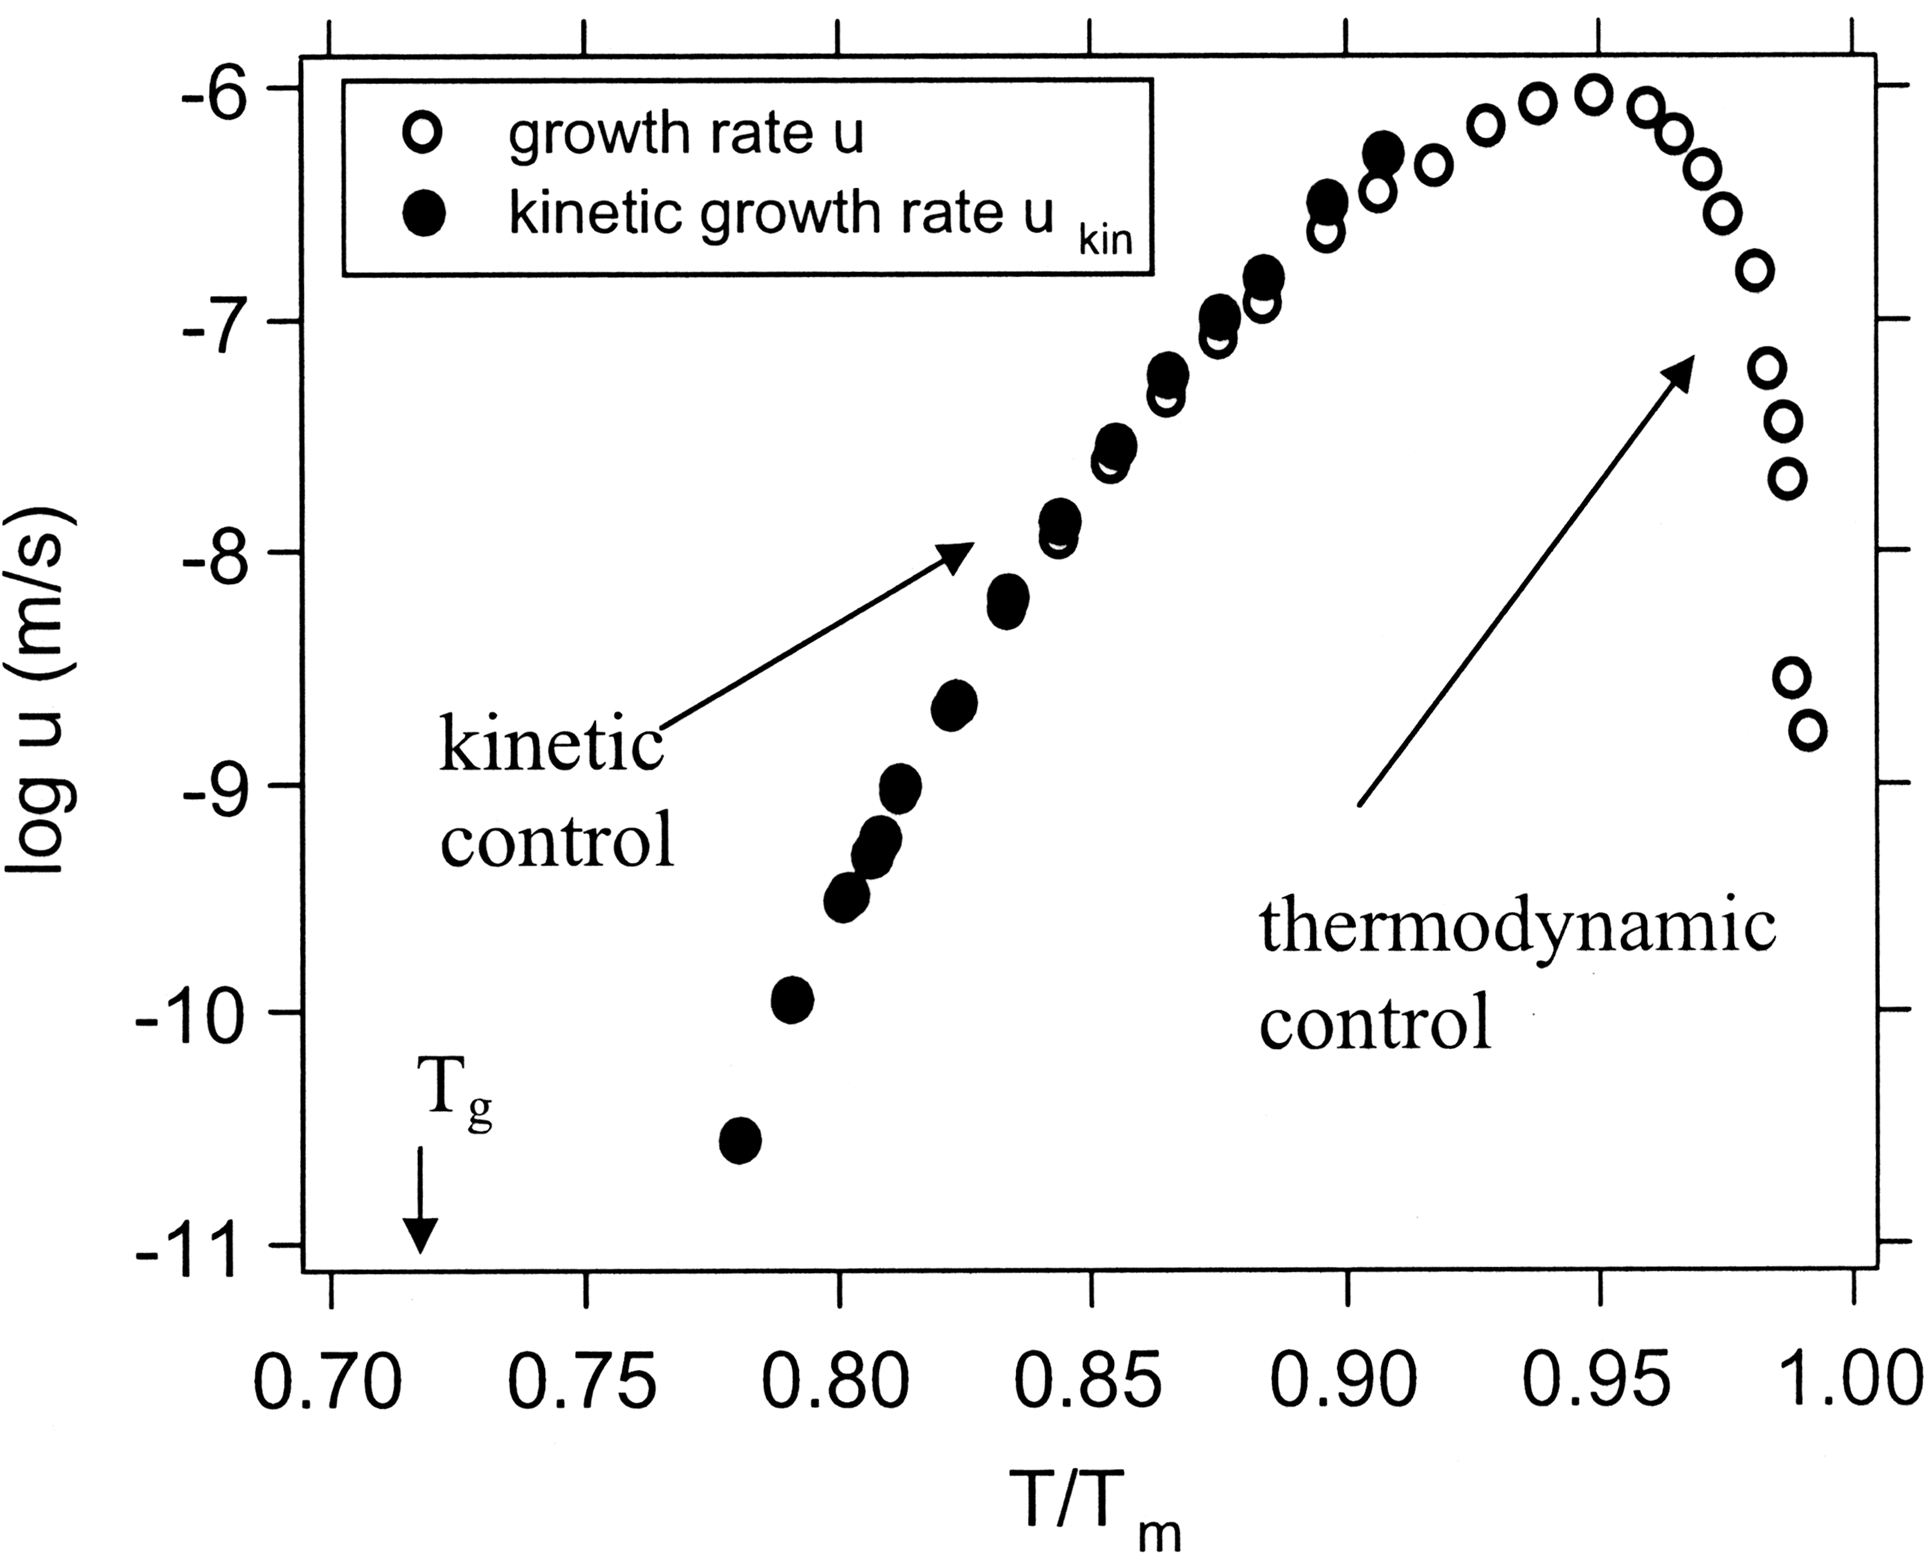
\includegraphics[width=0.6\textwidth]{crystal-growth}
    \caption[Crystal growth rate as a function of temperature]{Experimentally determined crystal growth rate as a function of temperature for supercooled tri-(napthylbenzene). As the temperature approaches \si{\Tg} the mobility of the liquid limits the rate at which the crystal can grow}
    \source{ediger:08}{AIP Publishing LLC}
    \label{fig:crys rate}
\end{figure}

If we are dealing with a system containing a constant number of particles, constant temperature and constant pressure, the standard conditions when working in a laboratory, the free energy that we are concerned with is the \emph{Gibbs free energy} ($G$). The change in free energy can be calculated using
\begin{equation}
    \Delta G = \Delta H - T\Delta S
\end{equation}
where $\Delta H$ is the change in enthalpy and $\Delta S$ is the change in entropy. At the melting point (\si{\Tm}) of a crystal $\Delta G = 0$, the temperature dependence on the entropy makes the liquid phase less favourable below the melting point; large supercoolings promote nucleation of the crystal phase. The entropy of the system is also a temperature dependent quantity which scales with the number of degrees of freedom~\figref{entropy}. In a crystal molecules are far more constrained than in a liquid giving the temperature dependence of entropy a more gradual slope~\figref{entropy}. The result of this is that if the supercooled liquid can be kept in the liquid state there is a point at which the entropy of the liquid is below that of the crystal. An important temperature when dealing with supercooled liquids is the \emph{glass transition temperature} (\si{\Tg}), defined as the temperature at which the viscosity of the supercooled liquid reaches \SI{e13}{\poise}. One of the theories of glass formation~\cite{debenedetti:01} is that the glass transition is the system providing a solution to the paradox, undergoing dynamical arrest above \si{\Tk} reducing the number of degrees of freedom.

\begin{figure}
    \centering
    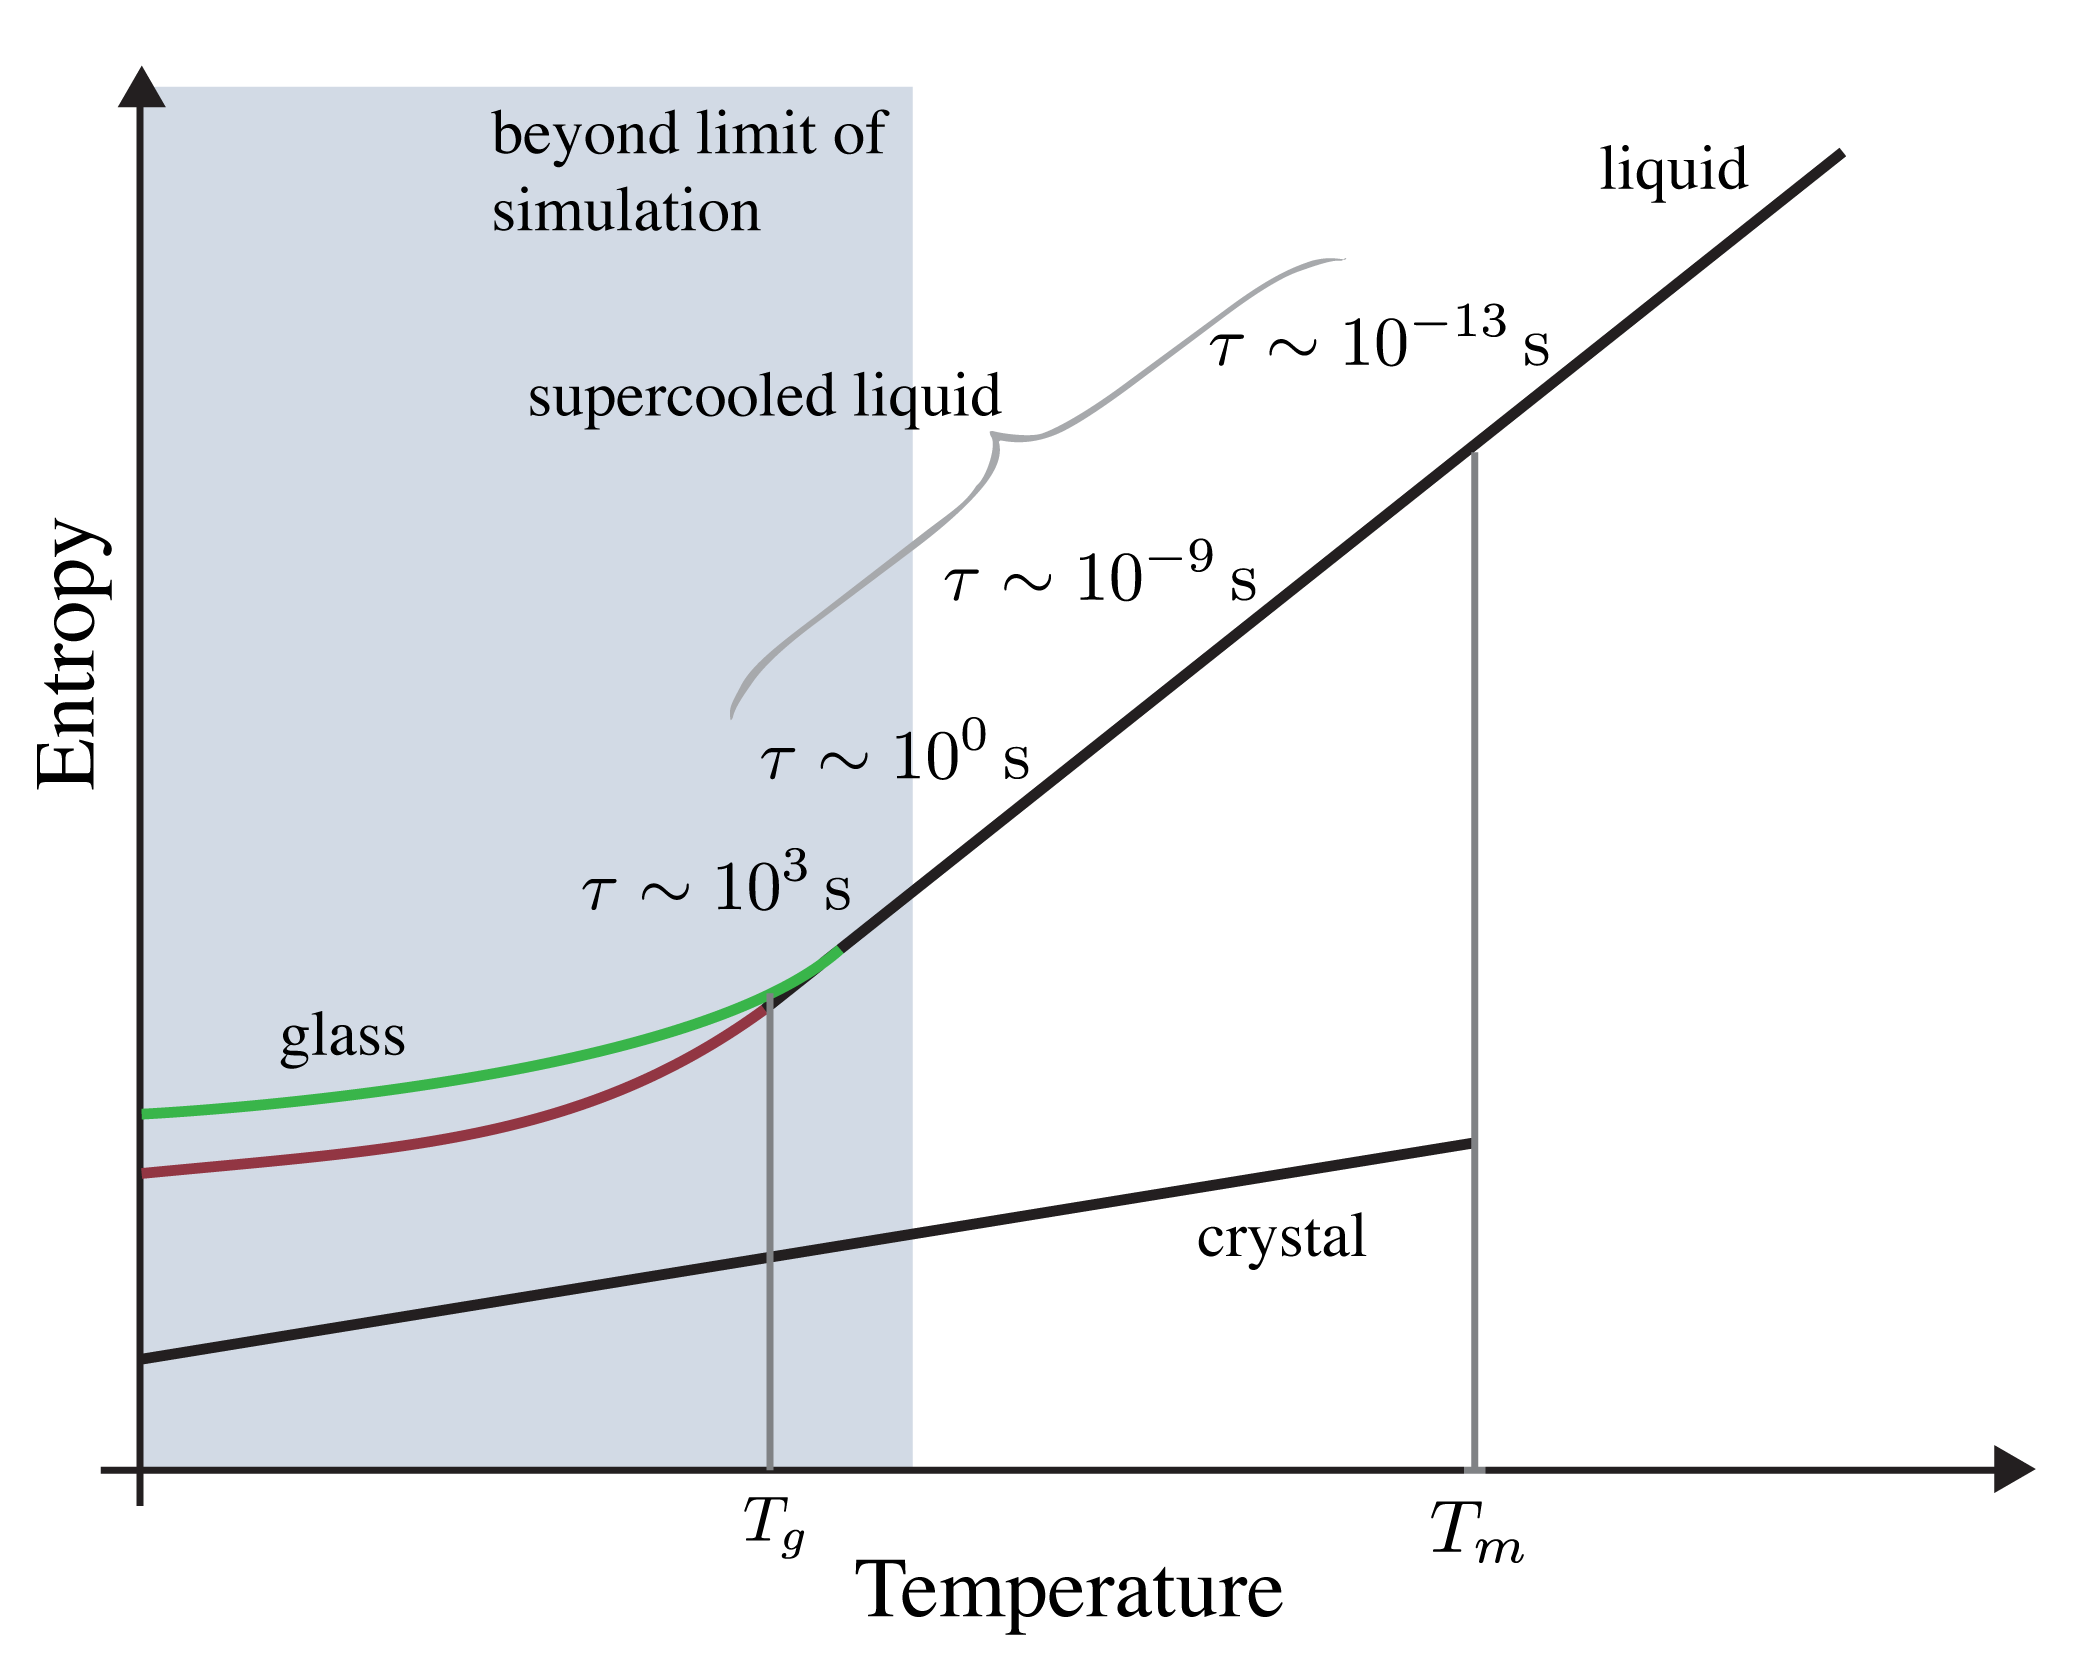
\includegraphics[width=0.6\linewidth]{supercooled}
    \caption{The temperature dependence of entropy for liquid, supercooled liquid, glass, and crystal phases. The liquid phases have more degrees of freedom and hence the larger slope. Note that the glass phase has relaxation time $\tau$ beyond the limit of current simulations.}
    \label{fig:entropy}
\end{figure}


When dealing with dynamics of supercooled liquids in most cases the viscosity observes Arrhenius behaviour just like a liquid. When approaching the glass transition temperature (\si{\Tg}) there are a number of supercooled liquids that display super-Arrhenius behaviour~\figref{angell} where there is a temperature dependence in the activation energy~\cite{angell:91}. Supercooled liquids that display this temperature dependence on the activation energy are known as \emph{fragile} liquids, they are interesting because they suggest that the glass transition temperature is not just an arbitrary concept but an inherent property of a material. The typical example of a fragile liquid is \emph{o}-terphenyl which has been widely studied~\cite{greet:67}. The liquids that keep the Arrhenius behaviour over the entire temperature range are known as \emph{strong} liquids, with the prototypical example being silica (\ce{SiO2}). The fragility ($m$) of a supercooled liquid can be given by the slope given in~\figref{angell},
\begin{equation}
    m = \left [ \pddiff{\log_{10} \eta}{\si{\Tg}/T} \right ]_{T=\si{\Tg}}
\end{equation}
This gives a range of fragilities from silica, $m = 22$ to \emph{o}-terphenyl, $m = 86$ with everything in between~\tabref{fragility}. It is interesting to note that along with \emph{o}-terphenyl many of the fragile supercooled liquids are molecular, this feeds the hypothesis that glass forming ability is in some way related to shape, it can not be the only contributing factor but is a line of investigation to pursue.

\begin{figure}
    \centering
    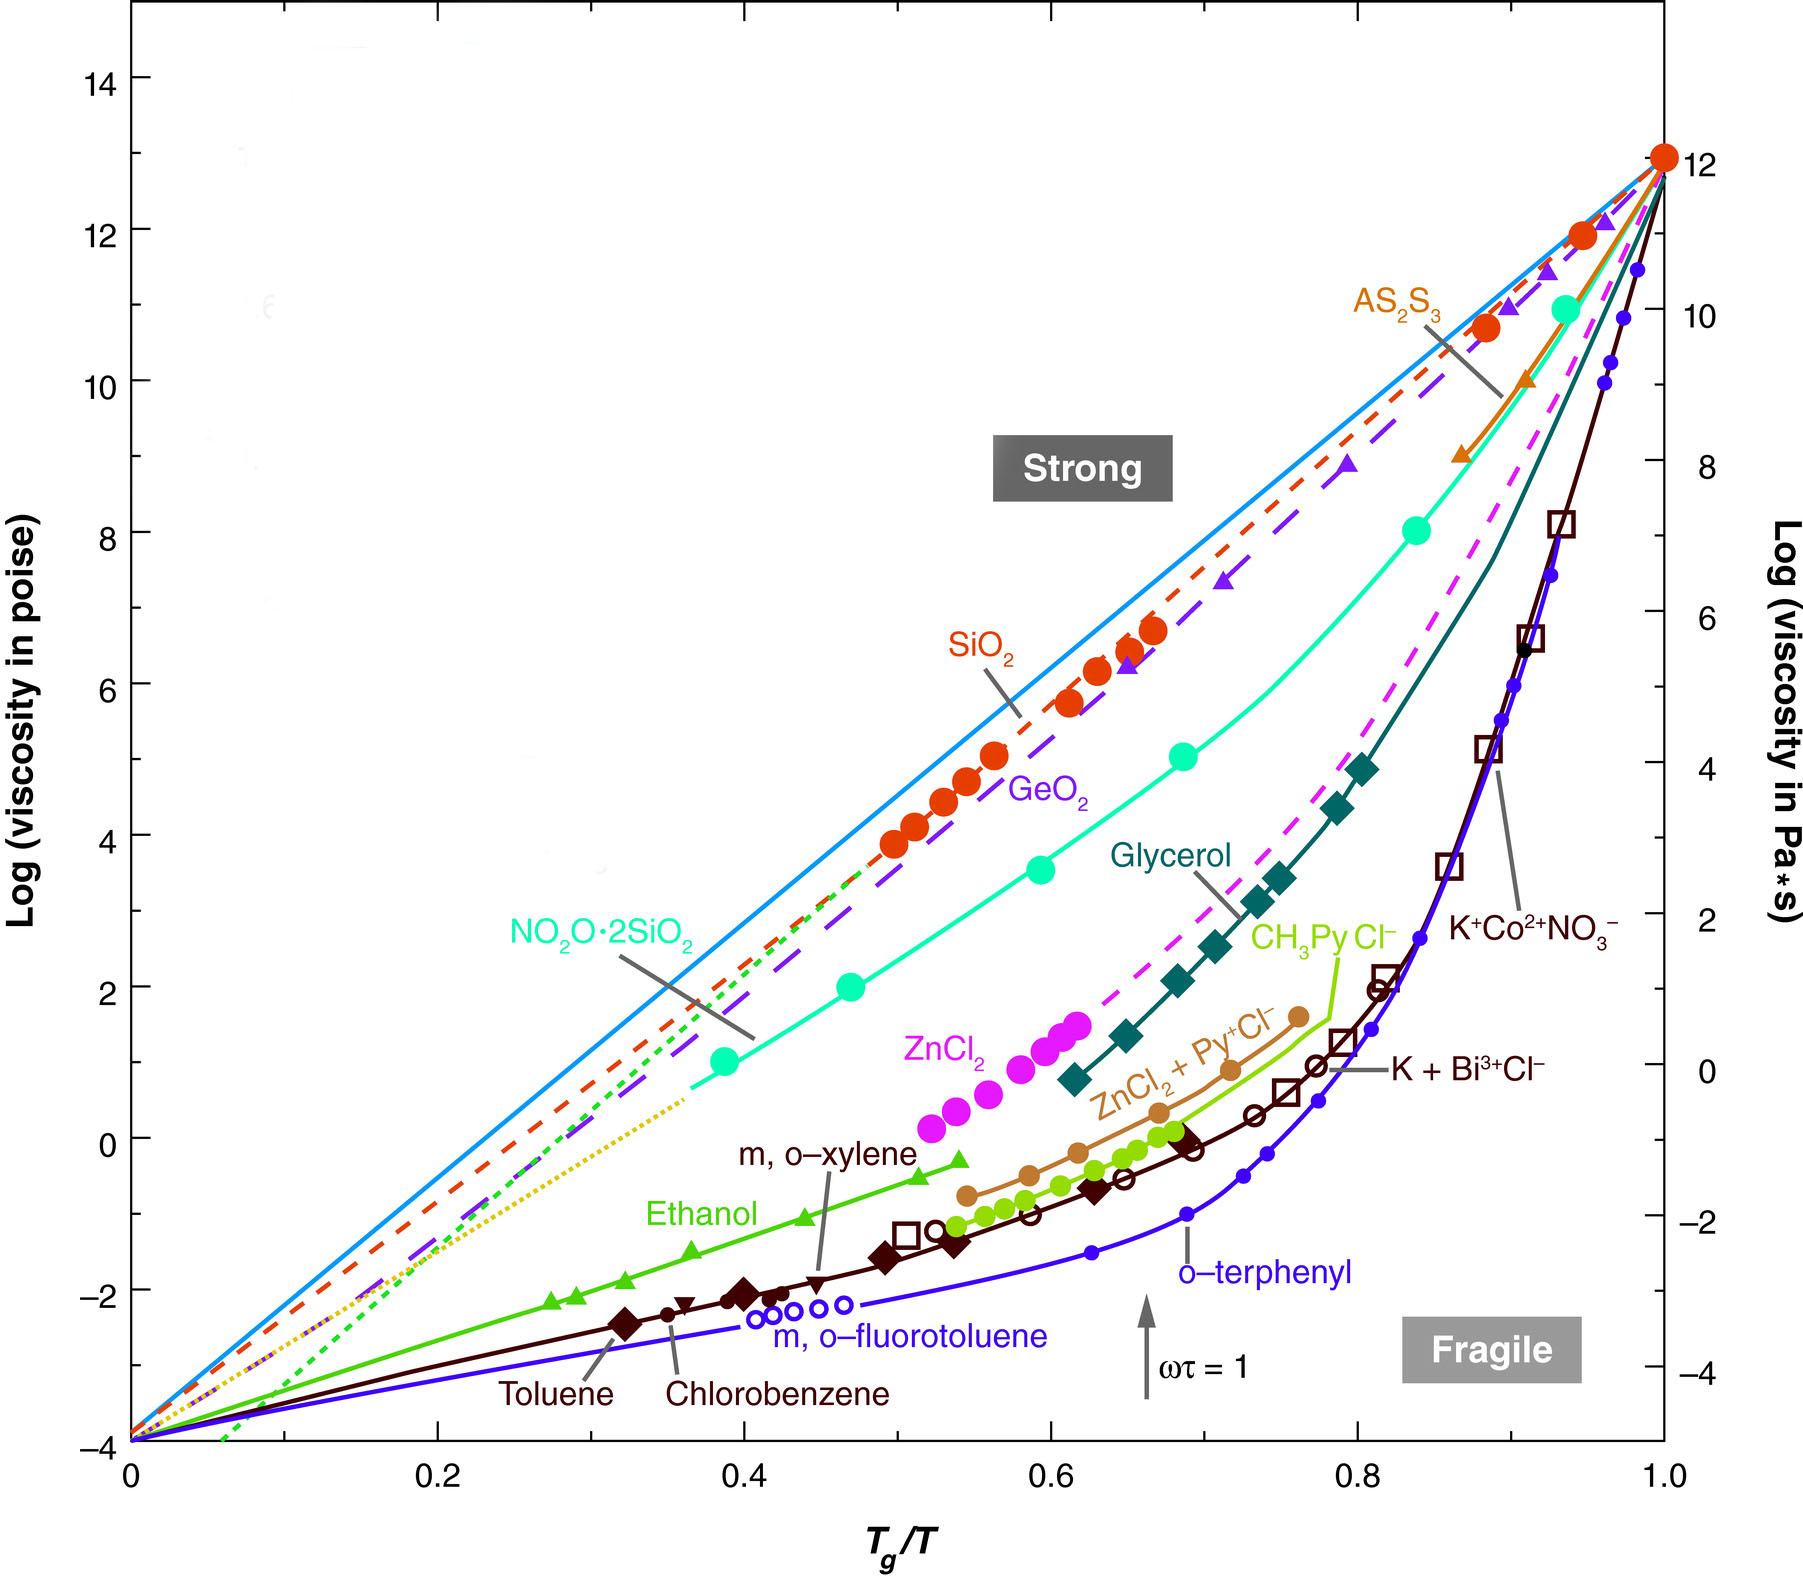
\includegraphics[width=\textwidth]{angell}
    \source{lubchenko:07}{Annual Reviews}
    \caption{Angell plot showing the relative response to cooling of a variety of glass formers.}
    \label{fig:angell}
\end{figure}

\begin{table}
    \begin{tabular}{| l | c c c |}
        \hline
        System & Fragility ($m$) & \si{\Tm} (\si{\kelvin}) & Type \\ \hline
        Indomethacin $\alpha$ (\ce{C_{19}H_{16}ClNO4}) & 89 & 426 & Molecular \\
        \emph{o}-terphenyl (\ce{C_{18}H_{14}}) & 86 & 329 & Molecular \\
        $\alpha$-phenol \emph{o}-cresol (\ce{C_{13}H_{14}O}) & 84 & 324 & Molecular \\
        Sorbitol E (\ce{C6H14O6}) & 77 & 353 & Molecular \\
        Diopside (\ce{CaO.MgO.2SiO2}) & 66 & 1664 & Ionic \\
        Sodium disilicate (\ce{Na2O.2SiO2}) & 45 & 1146 & Ionic \\
        Silica (\ce{SiO2}) & 21 & 2007 & Ionic \\
        \hline
    \end{tabular}
    \caption{The fragility of a number of different systems}
    \label{tab:fragility}
\end{table}

Along with the fragility of molecular glass formers, they are also interesting due to their rotational motion. In supercooled liquids below approximately \SI{1.2}{\Tg} there is a decoupling between rotational and translational diffusion~\cite{debenedetti:01,stillinger:95}. It has been found that molecules translate faster than expected for their viscosity by as much as two orders of magnitude~\cite{debenedetti:01}. This results in molecules being able to move past each other but unable to rotate, limiting the range of states that can be sampled by the supercooled liquid. This is not the only decoupling present as close to \si{\Tg}, there is also a splitting of the relaxation frequency into two bands, the slow $\alpha$ relaxation and fast $\beta$ relaxation~\tocite. This decoupling in the relaxation can be explained by interpreting the supercooled liquid as a point on a multidimensional potential energy landscape, just like for the packing problem~\secref{molecular crystals}. Here the way that the supercooled liquid moves through the potential energy landscape is a function of the temperature. At high temperatures the liquid moves freely about the potential energy landscape, the energy of the molecules is often above any of the potential energy barriers. As the temperature gets lower the space of configurations available to the system gets smaller, there are potential energy barriers a low probability of being crossed. Close to the glass transition temperature the space of configurations is limited, there are many small local potential energy minima separated by larger energy minima. Moving between these larger minima requires a large number of cooperative rearrangements in the structure of the system, these movements correspond to the slow $\alpha$ relaxations~\figref{pe landscape}. The motion between the smaller energy minima are the $\beta$ relaxations resulting from small particle shifts.

\begin{figure}
    \centering
    \todofigure{Potential energy landscape showing alpha a beta relaxations}
    \caption{}
    \label{fig:pe landscape}
\end{figure}

This topological view of the relaxation is consistent with a growing dynamic length scale, a property observed when approaching the glass transition~\cite{berthier:05}. At low temperatures the ability of the system to rearrange is very limited and requires coordinated rearrangement molecules to move between each of the larger potential energy wells. Moving back into real space this growing dynamic length scale was first theorised when looking at dynamic heterogeneity~\cite{hurley:95} in model glass formers. These simulations showed areas of glasses that were highly mobile, where other regions were completely stationary. The mobile regions are those that are cooperatively moving as the liquid relaxes. As the supercooled liquid moves to lower temperatures larger regions have to move cooperatively, in the topological view this is where there is a barrier that is insurmountable in one direction, however by incorporating more particles and increasing the dimensionality the supercooled liquid can just move around the barrier~\figref{barrier dimensions}.

\begin{figure}
    \centering
    \todofigure{Increasing dimensionality to go around barrier}
    \caption{In 2D space there is a barrier that is impassable, by including the 3rd dimension the traversal of the barrier is just a simple case of going around.}
    \label{fig:barrier dimensions}
\end{figure}

\section{Molecular Glasses}
\label{sec:molecular glasses}

The structure of a glass is indistinguishable from that of a liquid, the difference is that a glass has a viscosity of \SI{e13}{\poise}. Despite the liquid like structure, and urban legends~\tocite the glassy phase is most definitely solid, it would require a timescale of 100 million years for a glass with a viscosity at the glass transition to appreciably flow~\tocite. Much of the misunderstanding of the glassy phase is related to the lack of a first order phase transition~\tocite. None of the thermodynamic properties change upon transition, all the structural properties of the liquid phase apply to the glass phase, however the dynamics of the glass phase are far slower than any liquid.

Inherent structures are the structures generated when vibrations are removed, they are structures at a temperature of \SI{0}{\kelvin}. Removing vibrations is important for determining whether particles are within a cutoff to determine whether they are neighbours, the vibrations can be easily large enough to push molecules inside or outside this cutoff producing noisy results. By taking a number of inherent structures at various temperatures~\figref{inherent structures} the temperature dependence of inherent structure energy can be seen. This means that any glassy state is dependent on its temperature history, glasses cooled quickly have different properties to those cooled slowly.

At high temperature the liquid can sample the entire energy landscape where most of the energy minima are shallow giving high energy inherent structures. At low temperatures many of the energy minima are inaccessible, the energy required to reach them exceeds the energy of the system. In the case of the fast cooling the system is stuck with an energy barrier between the states it can occupy and the lower energy states being occupied by the slow cooling.

\begin{figure}
    \centering
    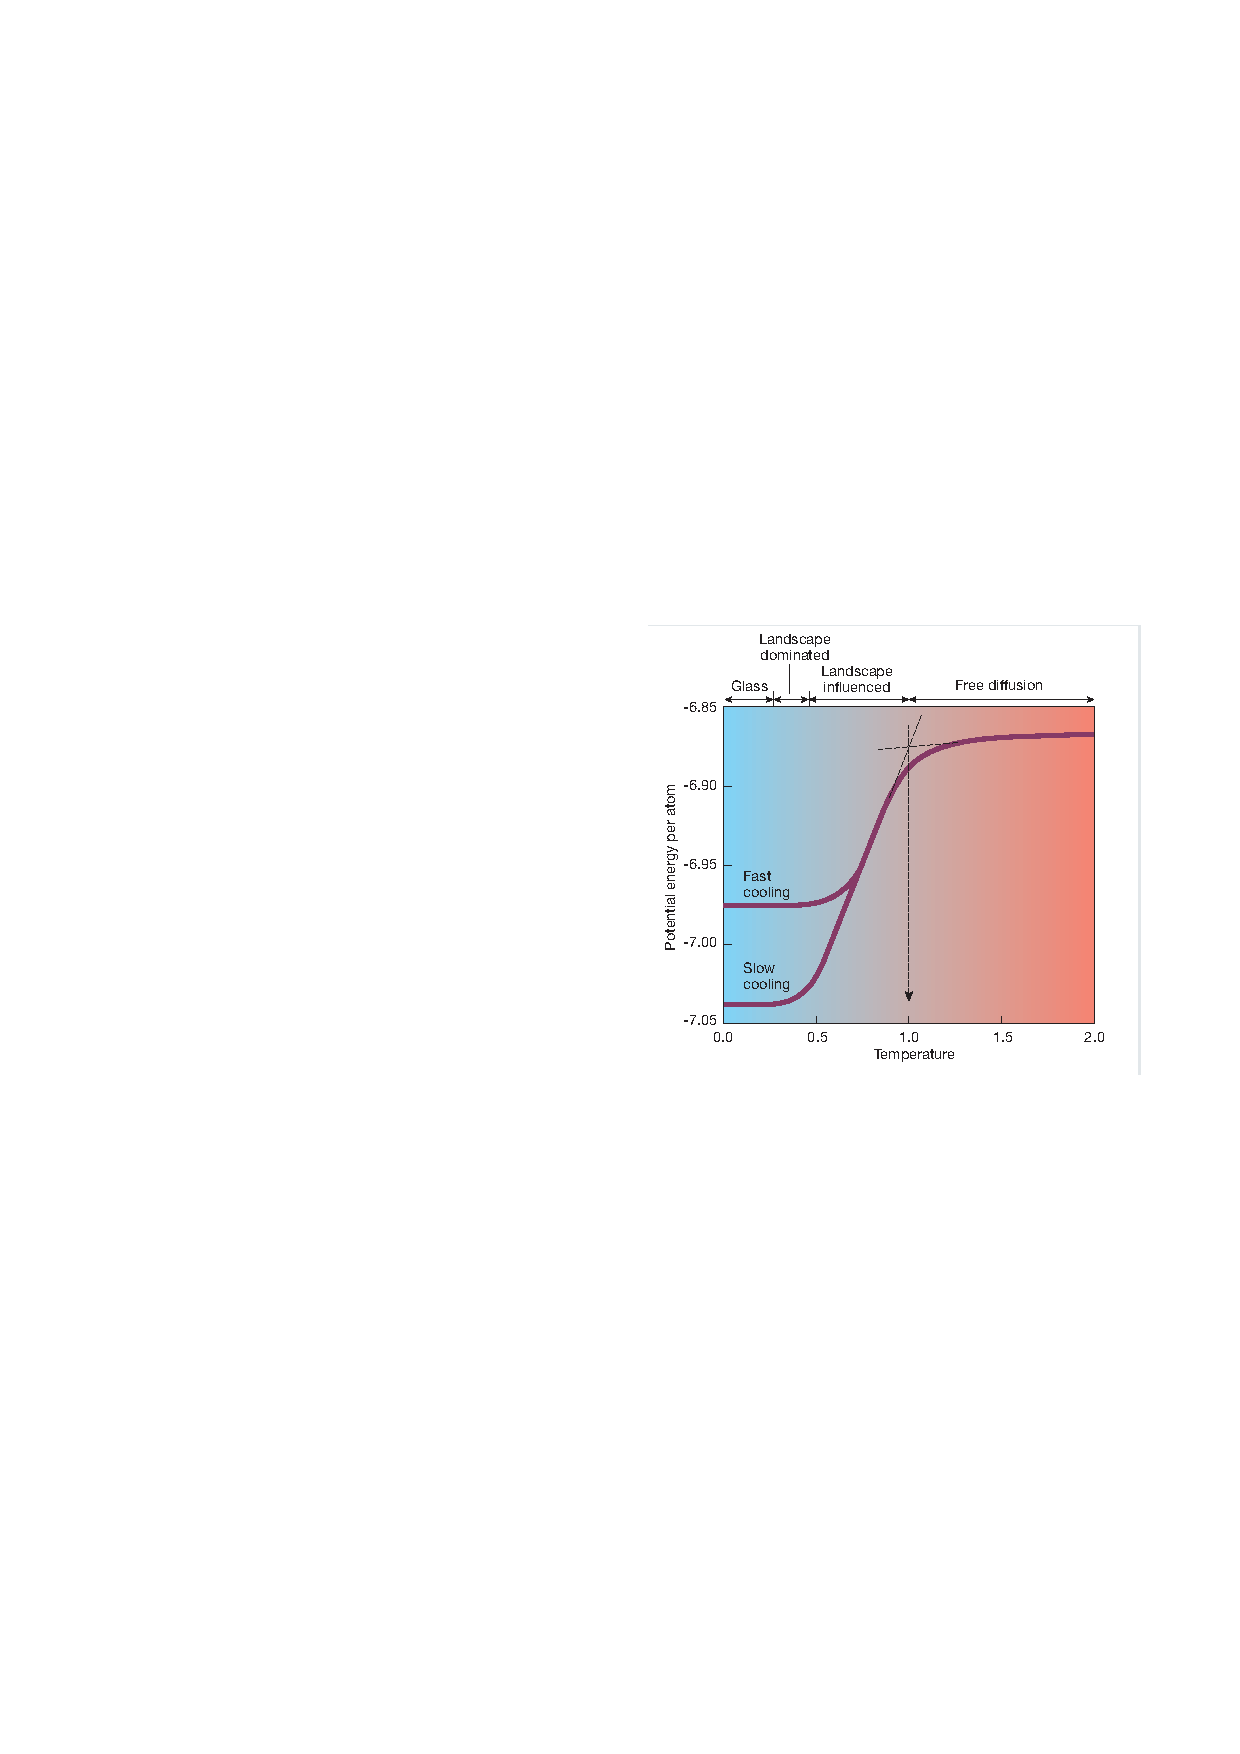
\includegraphics[width=0.75\linewidth]{inherent_structures}
    \caption[The mean inherent structure energy as a function of temperature]{The mean inherent structure energy per particle of a binary Lennard-Jones mixture as a function of the temperature of the equilibrated liquid from which the inherent structures were generated.}
    \source{debenedetti:01}{Nature Publishing Group}
    \label{fig:inherent structures}
\end{figure}

